\section*{Exercice 2 : Allocation M�moire (6 points)}

SunOS 5.4 introduit en 1994 un nouveau type d'allocateur m�moire grain fin
appel� ``slab allocator''.

Des allocateurs m�moire similaires ont ensuite �t� impl�ment�s dans Linux,
FreeBSD et beaucoup d'autres syst�mes d'exploitations.

Le principe de l'allocateur se base sur plusieurs hypoth�ses :
\begin{itemize}
  \item Les blocs de m�moire allou�s par l'utilisateur sont souvent de
        taille identique. Car la plupart du temps, ceux-ci correspondent
	a des objets pour le noyau.
  \item Lors de la lib�ration d'un objet, la lib�ration de la m�moire physique
        correspondante est pr�matur�e. Un comportement de cache est pr�f�rable.
  \item La gestion des structures internes de l'allocateur ne doit pas �tre
	plus lourde que l'allocation m�moire elle-m\^eme.
\end{itemize}

Cet allocateur est compos� d'objets appel�s ``caches'' et ``slabs''.
Un cache maintient une liste de slabs qu'il g�re. Un slab contient
physiquement un ensemble de blocs m�moire de taille identique.

Dans notre noyau exp�rimental chicheOS, nous disposons du code suivant :

\begin{lstlisting}

/* Objet cache */
typedef struct
{
  kmem_slab_t   *slab_list;     /* Liste de slabs du cache */
  kmem_slab_t   *free_slab;     /* Pointe vers un slab qui contient au moins
                                   un bloc libre */

  size_t        obj_size;       /* Taille des objets stockes dans les slabs du
                                   cache */

  ...

} kmem_cache_t;

/* Descripteur de slab */
typedef struct
{
  int           nobjs_max;      /* Nombre de blocs contenus dans le slabs */
  int           nobjs;          /* Nombre de blocs alloues */

  int	        first_free;	/* Index d'un bloc libre */

  char*         block_list;	/* Pointe vers la liste des blocs m�moire */
  int*	        free_list;	/* Tableau d'entiers contenant pour chaque bloc :
                                   -1 si le bloc est deja allou�
                                   l'index d'un autre bloc libre si le bloc
                                   est libre */

  kmem_slab_t   *next;          /* Liste doublement chain�e circulaire des */
  kmem_slab_t   *prev;          /* slabs du cache */

  kmem_cache_t  *cache;         /* Pointeur vers le cache qui possede ce slab */

} kmem_slab_t;

\end{lstlisting}

\newpage
On suppose que chaque slab occupe exactement 1 page m�moire de 4096 octets :

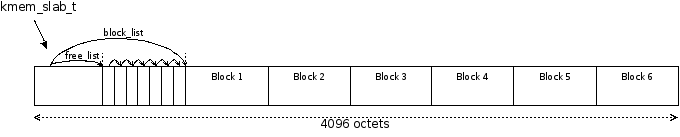
\includegraphics[width=\textwidth]{figures/slablayout.png}

\subsection*{Questions}

\begin{enumerate}
\item Vous disposez de \verb+kmem_cache_t * kmem_cache_region+, un pointeur vers
le cache qui g�re tout les objets de type \verb+region_t+.  �crivez la fonction
\verb+region_t * kmem_region_alloc()+ qui alloue un objet
\verb+region_t+ en m�moire. (Vous ne devez pas g�rer le cas d'ajout d'un slab dans le cache)
\item On souhaite lib�rer un objet \verb+region_t+ allou� pr�alablement par la fonction
\verb+kmem_region_alloc()+. Proposez une solution simple pour retrouver le slab
dans lequel se situe notre objet, \`a partir de son adresse.
\item Quels types d'objets ne peuvent pas �tre allou�s le slab allocator de ChicheOS ?
\item ChicheOS est �crit en C, n�ammoins, on souhaite pouvoir initialiser et nettoyer
le contenu des objets \verb+region_t+ lors de leur allocation et lib�ration.
Comment peut-on s'y prendre ?
\end{enumerate}

